%\documentclass[czech,12pt]{article}
\documentclass{beamer}
\usetheme{Madrid}
\setbeamertemplate{bibliography item}{[\theenumiv]} % cislovana bibliography
\setbeamertemplate{navigation symbols}{} % Odstranění navigační lišty. 

\usepackage[T1]{fontenc}
\usepackage[utf8]{inputenc}
\usepackage[czech]{babel}
\usepackage{graphicx}
\usepackage{hyperref}

\title{Kryptosystém McEliece}
\subtitle[]{Diplomová práce}
\author[Vojtěch Myslivec]{
Bc. Vojtěch Myslivec \\
\hfil \\
{\small vedoucí: prof. Ing. Róbert Lórencz, CSc.}
}
\institute[FIT ČVUT]{
   
\includegraphics[width=0.1\textwidth]{../materialy/cvut-logo-bw} \\
   \vspace{0.5cm}
   Fakulta informačních technologií \\
   České vysoké učení technické v~Praze\\
}
\date{\today}




\begin{document}

% ------------------------------------------------------------------------------
\begin{frame}[plain]
   \titlepage
\end{frame}

% ------------------------------------------------------------------------------
\begin{frame}{Obsah}
   \tableofcontents
\end{frame}

% ==============================================================================
% ==============================================================================
\section{Motivace}
% ------------------------------------------------------------------------------
\begin{frame}{Obsah}
    \tableofcontents[currentsection]
\end{frame}

% ------------------------------------------------------------------------------
\begin{frame}{Postkvantová kryptografie}
    \begin{itemize}

            \pause
        \item Kvantové počítače -- \alert{Shorův algoritmus} 1994.

            \pause
        \item \emph{RSA}, \emph{ECDSA}, \ldots

            \pause

        \item Kandidáti pro postkvantovou
            kryptografii~\cite{Post-Quantum_Cryptography,Schanck}.
            \begin{itemize}
                \item Symetrická kryptografie -- \emph{AES}
                \item \emph{Lattice-based} (svaz)
                \item \emph{Hash-based}
                \item \emph{Code-based}
                    \pause
                    -- \alert{McEliece}
            \end{itemize}
    \end{itemize}
\end{frame}

% ==============================================================================
% ==============================================================================
\section{Popis kryptosystému}
% ------------------------------------------------------------------------------
\begin{frame}{Obsah}
    \tableofcontents[currentsection]
\end{frame}

% ------------------------------------------------------------------------------
\begin{frame}{Kryptosystém McEliece}
    \begin{itemize}

        \item \emph{Robert McEliece} 1978~\cite{McEliece}.
        \item Systém pro \structure{asymetrické šifrování}.

            \pause
        \item Využívá \structure{lineární kód} pro opravu chyb.

            \begin{itemize}
                \item Náhodný \structure{chybový vektor} jako součást šifry.
                \item Dekódovat neznámý lineární kód je \structure{NP-těžká}
                    úloha~\cite{Berlekamp1}.
            \end{itemize}

            \pause
        \item \alert{Velké klíče} (stovky kilobitů až jednotky megabitů).

    \end{itemize}
\end{frame}

% ==============================================================================
\subsection{Generování klíčů}
% ------------------------------------------------------------------------------
\begin{frame}{Generování klíčů}

        \pause
    \begin{block}{Generování klíčů}
        \begin{enumerate}

            \item \emph{Lineární kód}~$\mathcal{K}$ $(n,k)$
                opravující~$t$ chyb, s~$k \times n$ \alert{generující
                maticí~$G$}.
            \item Náhodná $k \times k$ \alert{regulární matice $S$}.
            \item Náhodná $n \times n$ \alert{permutační matice $P$}.
            \item Vypočítáme $k \times n$ matici $\hat{G} = S G P$.

        \end{enumerate}
    \end{block}

        \pause
    \begin{block}{Vygenerované klíče}
        \begin{itemize}
            \item[] \textbf{Veřejné parametry} \hfil \\
                \hspace{0.5cm} Čísla $k, n, t$
            \item[] \textbf{Veřejný klíč} \hfil \\
                \hspace{0.5cm} Matice $\hat{G}$ ($\hat{G} = S G P$)
            \item[] \textbf{Soukromý klíč} \hfil \\
                \hspace{0.5cm} Matice $S, P$ a kód $\mathcal{K}$ generovaný $G$.
        \end{itemize}
    \end{block}

\end{frame}


% ==============================================================================
\subsection{Algoritmy pro šifrování a dešifrování}
% ------------------------------------------------------------------------------
\begin{frame}{Algoritmy}

    \begin{block}{Šifrování}
        \textbf{Algoritmus $E$:} \\
        Máme zprávu $m$ délky $k$, veřejný klíč $\hat{G}$ a parametr $t$.
        \begin{enumerate}
            \item Vygenerujeme chybový vektor $z$ délky $n$ s~\emph{Hammingovou
                vahou} $t$.
            \item Šifrový text $c = m \hat{G} + z$.
        \end{enumerate}
    \end{block}

\pause

    \begin{block}{Dešifrování}
        \textbf{Algoritmus $D$:}
        \begin{enumerate}
            \item Vypočítáme $\hat{c} = c P^{-1}$.
            \item Dekódujeme $\hat{m}$ z~$\hat{c}$ pomocí použitého kódu. \\
                $Dek(\hat{c}) = \hat{m}$
            \item Vypočítat původní zprávu $m = \hat{m} S^{-1}$.
        \end{enumerate}
    \end{block}

\end{frame}

% ==============================================================================
% ==============================================================================
\section{Binární Goppa kódy}
% ------------------------------------------------------------------------------
\begin{frame}{Obsah}
    \tableofcontents[currentsection]
\end{frame}

% ------------------------------------------------------------------------------
\begin{frame}{Binární Goppa kódy}
    \begin{itemize}

        \item \emph{Valery Goppa} 1970~\cite{Goppa}.
        \item Nová kategorie \emph{lineárních kódů} -- AG kódy $\sim$ Goppa kódy.

            \pause
        \item Neexistují útoky na strukturu kódu.

            \pause
        \item Základ pro \emph{code-based} kryptografii.

    \end{itemize}
\end{frame}

% ==============================================================================
\subsection{Sestrojení binárního Goppa kódu}
% ------------------------------------------------------------------------------
\begin{frame}{Binární Goppa kódy}

    \begin{block}{Sestrojení binárního (ireducibilního) Goppa kódu}
        Kód $\Gamma$ s~parametry $(n,k)$ opravující $t$ chyb.
        \begin{itemize}

        \pause
            \item \textbf{Goppův polynom $g$} \\
                (Ireducibilní) polynom stupně $t$ z~okruhu polynomů nad
                konečným tělesem $\mathbb F = GF(2^m)$
                $$ g \in \mathbb F [x] \quad deg(g) = t $$

        \pause
            \item \textbf{Podpora $L$} \\
                Posloupnost $n$ různých prvků z~tělesa $\mathbb F$, které
                nejsou kořenem $g$
                $$
                    L = \left( L_1, \ldots, L_n \right) \quad \forall i,j : L_i \in
                    \mathbb{F} \land L_i \neq L_j \land g(L_i) \neq \mathbf{0}
                $$

        \pause
            \item \textbf{Kontrolní matice $H$} \\
                pokračování \ldots
        \end{itemize}
    \end{block}

\end{frame}

% ------------------------------------------------------------------------------
\begin{frame}{Binární Goppa kódy}

    \begin{block}{Sestrojení binárního (ireducibilního) Goppa kódu}
        \begin{itemize}

            \item \textbf{Kontrolní matice $H$} \\
                $$ H = V D $$

            \pause
            %\emph{Vandermondova} matice $V$
                $$
                    V = \left(\begin{array}{c c c c}
                        1         & 1         & \ldots & 1         \\
                        L_1       & L_2       & \ldots & L_n       \\
                        \vdots    & \vdots    & \ddots & \vdots    \\
                        L_1^{t-1} & L_2^{t-1} & \ldots & L_n^{t-1} \\
                    \end{array}\right)
                $$

            \pause
            %\emph{Diagonální} matice $D$
                $$
                    D = \left(\begin{array}{c c c c}
                        g(L_1)^{-1} &             &        &             \\
                                    & g(L_2)^{-1} &        &             \\
                                    &             & \ddots &             \\
                                    &             &        & g(L_n)^{-1} \\
                    \end{array}\right)
                $$

        \end{itemize}
    \end{block}

\end{frame}


% ==============================================================================
\subsection{Dekódování}
% ------------------------------------------------------------------------------
\begin{frame}{Binární Goppa kódy}

    \begin{block}{Dekódování}
        \pause
        \emph{Pattersonův algoritmus}~\cite{Patterson}
            \pause
        \begin{itemize}
            \item Opravuje až $t$ chyb.
            \item Kritická místa:
                \begin{itemize}
                    \item Výpočet odmocniny.
                    \item Hledání kořenů.
                \end{itemize}
            \pause
            \item Detaily v~práci.
        \end{itemize}

    \end{block}

\end{frame}


% ==============================================================================
% ==============================================================================
\section{Implementace}
% ------------------------------------------------------------------------------
\begin{frame}{Obsah}
    \tableofcontents[currentsection]
\end{frame}

% ------------------------------------------------------------------------------
\begin{frame}{Implementace}

    \begin{itemize}
        \item Software \emph{Wolfram Mathematica}.
        \item Implementace rozdělena do samosataných \emph{balíků}.
        \item Implementováno:
            \begin{itemize}
                \item Funkce pro operace v~konečných tělesech (včetně
                    rozšířených).
                \item Goppa kódy
                \item McEliece
            \end{itemize}
    \end{itemize}
\end{frame}

% ------------------------------------------------------------------------------
\begin{frame}{Ukázka}

\end{frame}


% ==============================================================================
% ==============================================================================
\section{Shrnutí}
% ------------------------------------------------------------------------------
\begin{frame}{Obsah}
    \tableofcontents[currentsection]
\end{frame}

% ------------------------------------------------------------------------------
\begin{frame}{Shrnutí}
    \begin{block}{Práce se zabývá:}
            \begin{itemize}
                    \pause
                \item Popisem kryptosystému, včetně varianty pro digitální
                    podpis.
                    \pause
                \item Goppa kódy.
                    \pause
                \item Rozborem existujících kryptoanalýz a útoků.
                    \pause
                \item Moderními variantami a metodami na zkrácení klíčů.
                    \pause
                \item Implementací a měřením asymptotických složitostí.
            \end{itemize}
    \end{block}
\end{frame}


% ==============================================================================
% ==============================================================================
\section*{Otázky}
% ------------------------------------------------------------------------------
\begin{frame}{Otázky}

    \begin{center}
        \large Prostor pro otázky.
    \end{center}

        \pause
    Otázky oponenta:

    \begin{enumerate}

            \pause
        \item Má vůbec smysl hledat úsporu prostoru u~soukromého klíče,
            i~s~ohledem na vaše tvrzení, že kapacity disků jsou téměř neomezené
            a~limit je primárně v~přenosu veřejného klíče?

            \pause
        \item Zkoušel jste změřit dobu generování klíčů, šifrování a~dešifrování
            pro bezpečné parametry, tedy např. $m=12$, $t=41$?

    \end{enumerate}


\end{frame}

% ------------------------------------------------------------------------------
\begin{frame}{Otázky}

    \begin{block}{2. rozumné parametry}

        \begin{figure}
            \centering
            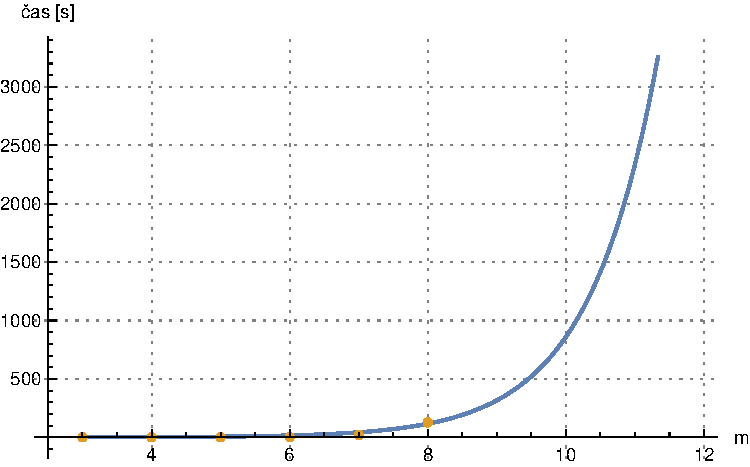
\includegraphics[width=0.7\textwidth]{../../implementace/grafy/extrapolace_generovani.pdf}
            \caption{Extrapolace doby trvání generování klíčů v~závislosti
            na~$m$.}
        \end{figure}
    \end{block}
\end{frame}

% ==============================================================================
% ==============================================================================
\section*{Reference}
% ------------------------------------------------------------------------------
\begin{frame}{Reference}
    \begin{thebibliography}{99}

    \bibitem{McEliece}
        Robert J. \textsc{McEliece}. A~Public-Key Cryptosystem Based on
        Algebraic Coding Theory v~\emph{JPL Deep Space Network Progress Report},
        strany 114-116. 1978. Dostupné online
        \url{http://ipnpr.jpl.nasa.gov/progress_report2/42-44/44N.PDF}

    \bibitem{Berlekamp1}
        Elwyn R. \textsc{Berlekamp}, Robert J. \textsc{McEliece}, Henk C. A. van
        \textsc{Tilborg}.  On the Inherent Intractibility v~\emph{IEEE
        Transactions of Information Theory}, vol. IT-24, No. 3, strany 384-386.
        IEEE, květen 1978.

    \bibitem{Post-Quantum_Cryptography}
        Daniel J. \textsc{Bernstein}, Johannes \textsc{Buchmann}, Erik
        \textsc{Dahmen}. \emph{Post-Quantum Cryptography}. ISBN
        978-3-540-88701-0.  Springer Berlin Heidelberg, 2009.

    \bibitem{Schanck}
        J. M. Schanck, W. Whyte, Z. Zhang. Criteria for selection of public-key
        cryptographic algorithms for quantum-safe hybrid cryptography
        (Internet-draft). IETF, 2016. Dostupné online
        \url{https://datatracker.ietf.org/doc/draft-whyte-select-pkc-qsh/}

    \bibitem{Goppa}
        Valery D. \textsc{Goppa}. A~New Class of Linear Correcting Codes
        v~\emph{Problemy Peredachi Informatsii}, vol. 6, strany 24-30. 1970.

    \bibitem{Patterson}
        Nicholas J. \textsc{Patterson}, The algebraic decoding of Goppa codes
        v~\emph{IEEE Transactions on Information Theory}, vol. 21, strany
        203-207. IEEE 1975. Dostupné online
        \url{http://ieeexplore.ieee.org/xpl/articleDetails.jsp?arnumber=1055350}

    \end{thebibliography}

\end{frame}

\end{document}


